\documentclass[11pt]{article}
\usepackage[margin=1in]{geometry}
\usepackage{times}
\usepackage{graphicx}
\usepackage{subcaption}
\usepackage[numbers]{natbib}
\bibliographystyle{plainnat}

\graphicspath{{figures/}}

\begin{filecontents}{references.bib}
@article{lecun1989backpropagation,
  title={Backpropagation applied to handwritten zip code recognition},
  author={LeCun, Yann and Boser, Bernhard and Denker, John S and Henderson, Donnie and Howard, Richard E and Hubbard, Wayne and Jackel, Lawrence D},
  journal={Neural computation},
  volume={1},
  number={4},
  pages={541--551},
  year={1989},
  publisher={MIT Press}
}
@inproceedings{vaswani2017attention,
  title={Attention is all you need},
  author={Vaswani, Ashish and Shazeer, Noam and Parmar, Niki et al.},
  booktitle={Advances in Neural Information Processing Systems (NeurIPS)},
  pages={5998--6008},
  year={2017}
}
@inproceedings{brown2020gpt3,
  title={Language Models are Few-Shot Learners},
  author={Brown, Tom B and Mann, Benjamin and Ryder, Nick et al.},
  booktitle={Advances in Neural Information Processing Systems (NeurIPS)},
  year={2020}
}
\end{filecontents}

\title{\bf Zero-Shot Neural-Symbolic Reasoning\newline in Real-World Pitfalls}
\author{Anonymous Submission}
\date{}

\begin{document}

\maketitle

\begin{abstract}
We investigate the challenges of zero-shot neural-symbolic generalization to unseen logical rules. Despite strong performance on training and validation data, our models fail to generalize to novel configurations. We highlight overfitting tendencies, illustrate how token-level biases arise, and reveal architectural sensitivities that harm the real-world deployment of these systems.
\end{abstract}

\section{Introduction}
Neural symbolic learning holds promise for systematically dealing with tasks requiring discrete reasoning~\citep{lecun1989backpropagation,vaswani2017attention}. Yet real-world scenarios demand robust zero-shot generalization to unseen rules. We show crucial pitfalls and negative results. Although training and validation performance appear reasonable, test accuracy on truly novel symbolic manipulations often collapses. Our main contributions include: (a) an empirical analysis of overfitting to known rules, (b) ablation studies revealing architecture sensitivities, (c) lessons drawn from negative outcomes for designing more robust models.

\section{Related Work}
Prior efforts have aimed to combine differentiable modules with symbolic reasoning, but many disregard systematic extrapolation~\citep{brown2020gpt3}. Recent approaches rely on encoder-decoder Transformers~\citep{vaswani2017attention}, yet few openly address negative outcomes or the difficulty in extrapolating to new symbolic transformations.

\section{Method / Problem Discussion}
We train Transformers to map input strings of symbolic expressions to specified transformations. We emphasize challenges: models that memorize training patterns fail on new symbolic rules. We systematically vary architecture components (positional embeddings, token pooling) to assess generalization.

\section{Experiments}
Our experiments were run on synthetic tasks where each sample is a symbolic expression. Figures~\ref{fig:baseline_training} and~\ref{fig:baseline_test} illustrate model performance.

\begin{figure}[ht]
  \centering
  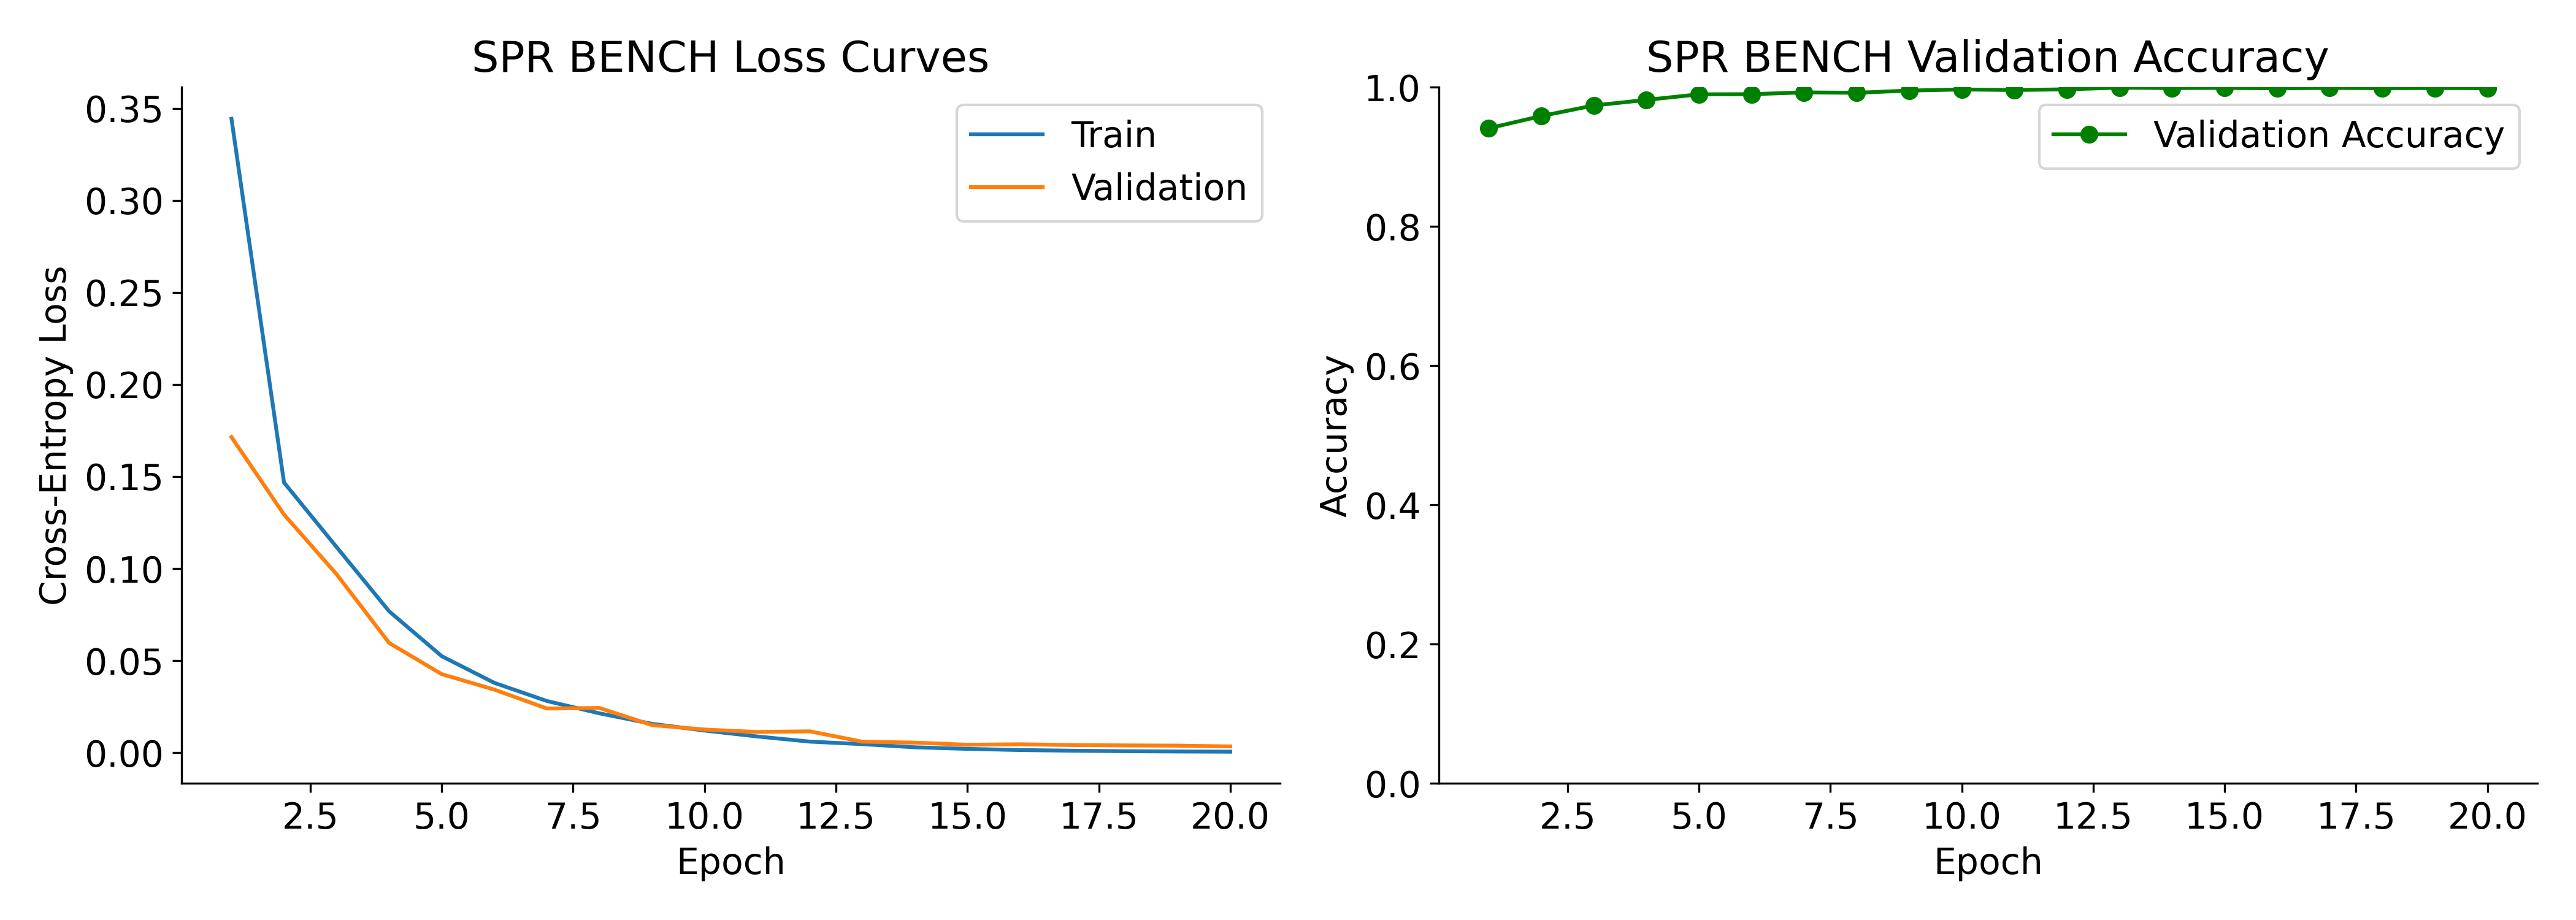
\includegraphics[width=0.65\linewidth]{baseline_loss_and_val_accuracy.png}
  \caption{Training curves and validation accuracy. Notice consistently declining loss with near-perfect validation performance.}
  \label{fig:baseline_training}
\end{figure}

\begin{figure}[ht]
  \centering
  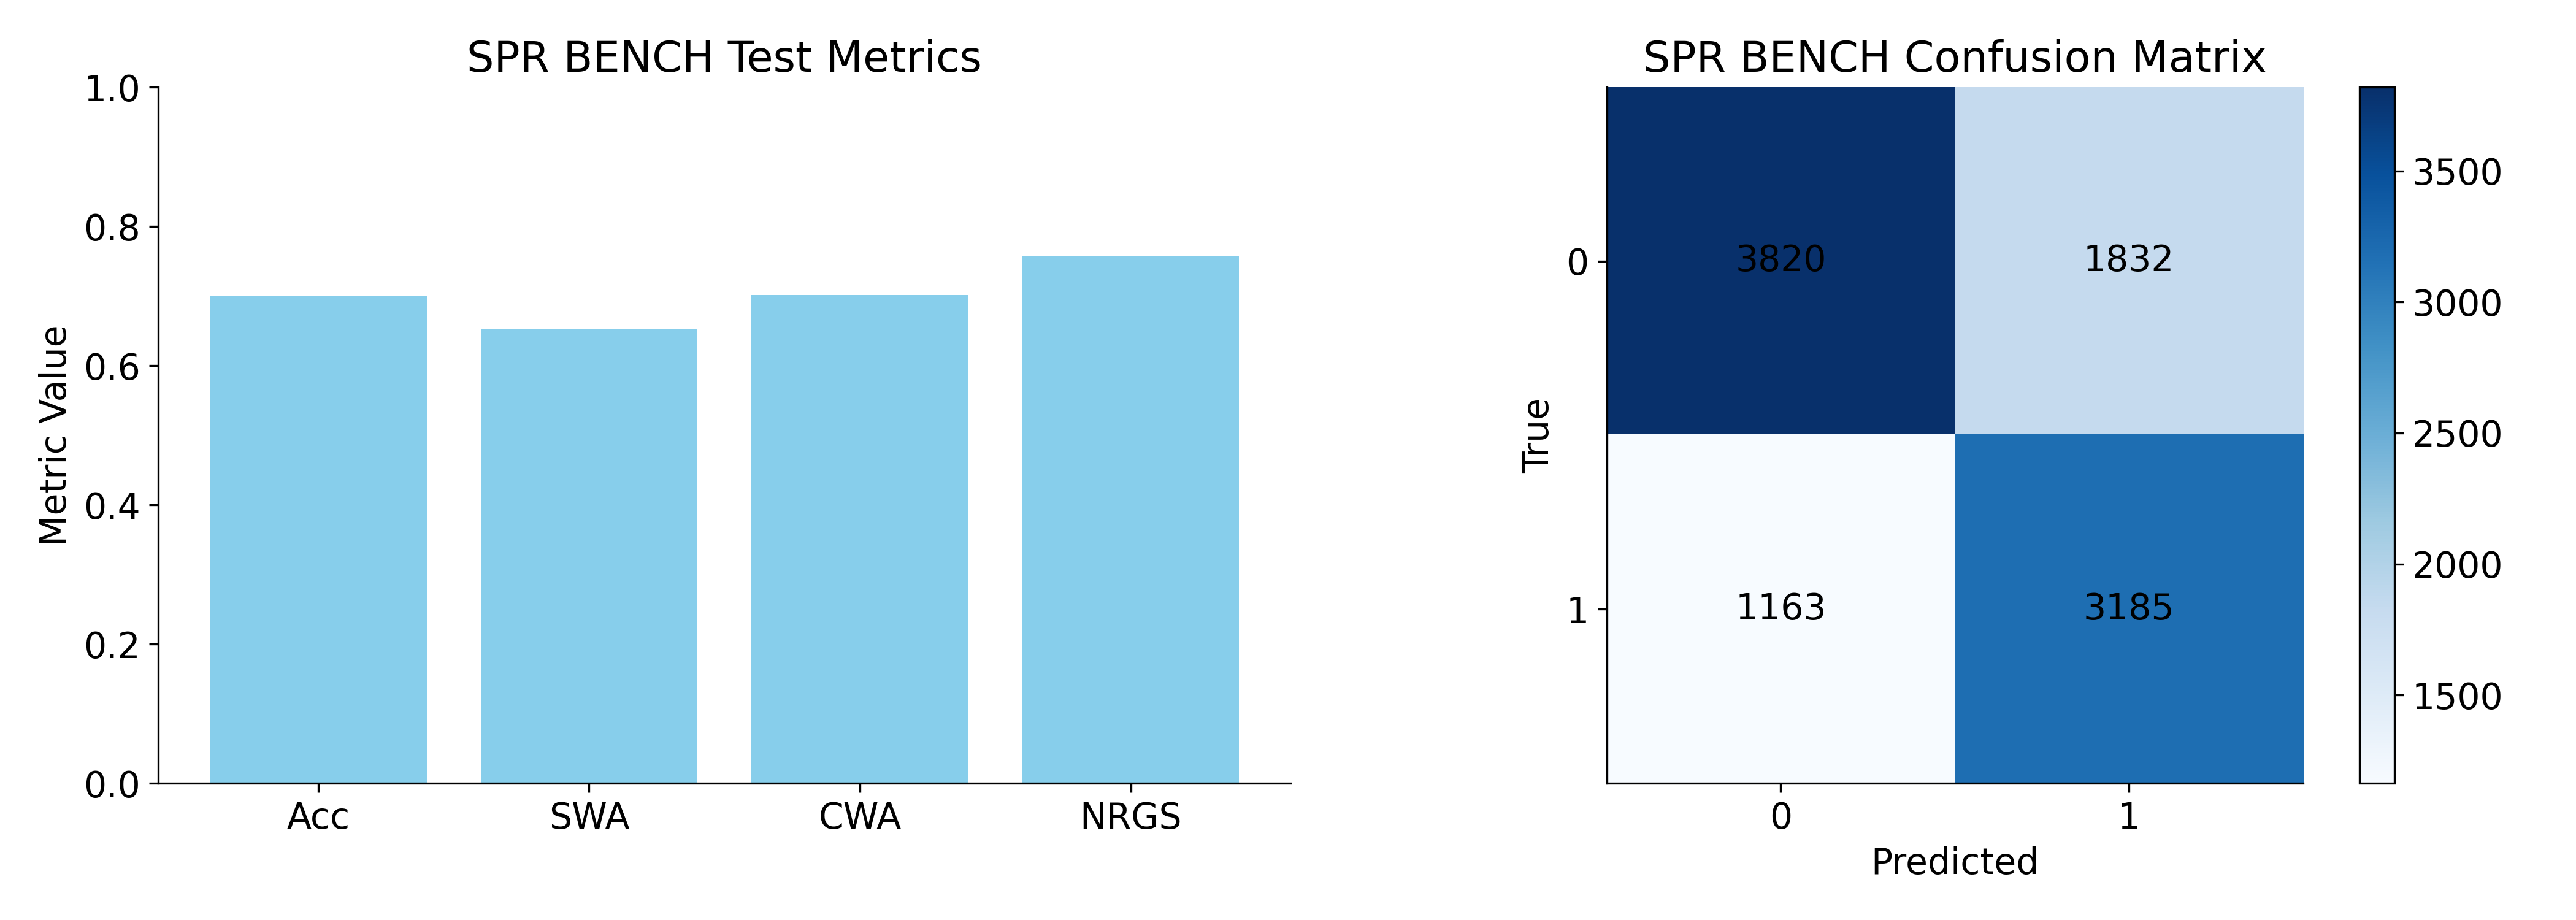
\includegraphics[width=0.6\linewidth]{baseline_test_metrics_and_confusion.png}
  \caption{Test metrics on unseen symbolic rules. Large gaps suggest overfitting to known configurations.}
  \label{fig:baseline_test}
\end{figure}

Substantial performance drops occur when encountering logic rules outside the training distribution. Our ablation results (Appendix) show sensitivity to embedding strategies, indicating partial successes but mostly highlighting limited capacity to extrapolate.

\section{Conclusion}
Zero-shot neural-symbolic reasoning for unseen logical rules largely remains unsolved. Despite strong training/validation results, generalization to novel structures is poor. We encourage direct evaluations on true unseen tasks and more rigorous architectures that could mitigate overfitting.

\clearpage
\appendix
\section{Supplementary Material}
\begin{figure}[ht]
  \centering
  \begin{subfigure}[b]{0.45\textwidth}
    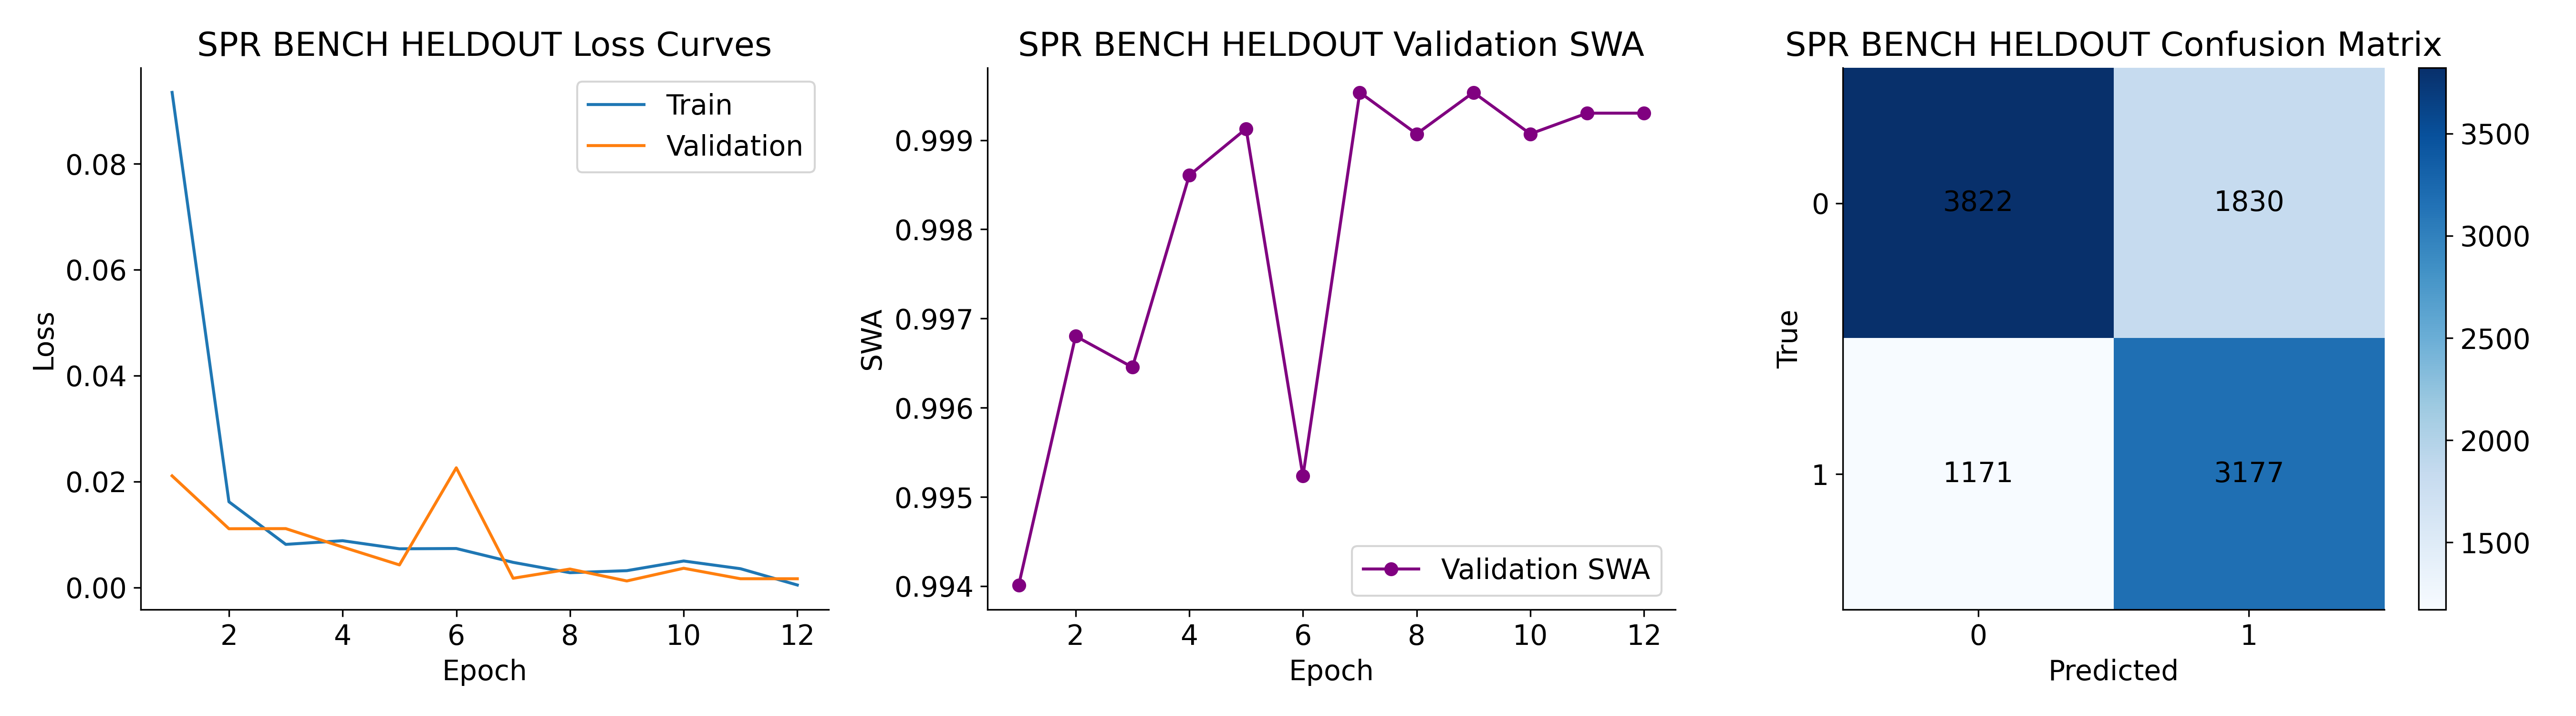
\includegraphics[width=\linewidth]{ablation_multidataset.png}
    \caption{Multi-dataset ablation.}
  \end{subfigure}
  \begin{subfigure}[b]{0.45\textwidth}
    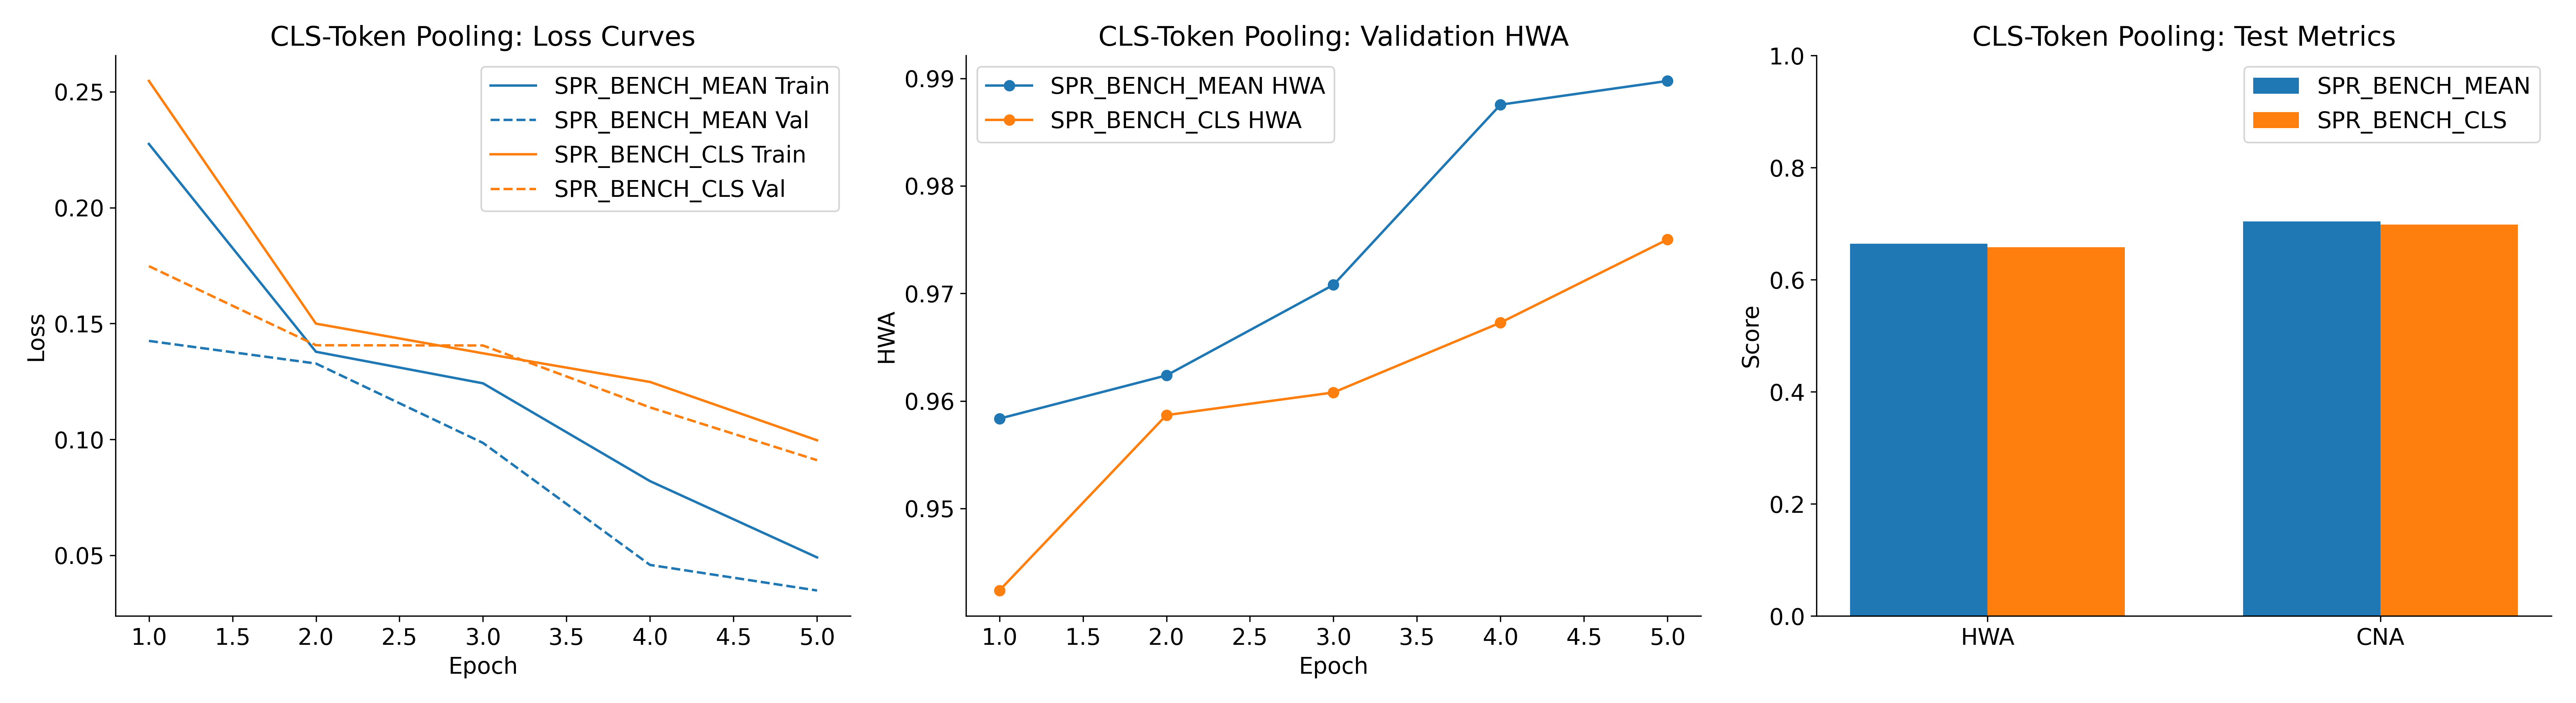
\includegraphics[width=\linewidth]{ablation_cls_token_pooling.png}
    \caption{Effect of CLS-token pooling.}
  \end{subfigure}
  \\
  \begin{subfigure}[b]{0.45\textwidth}
    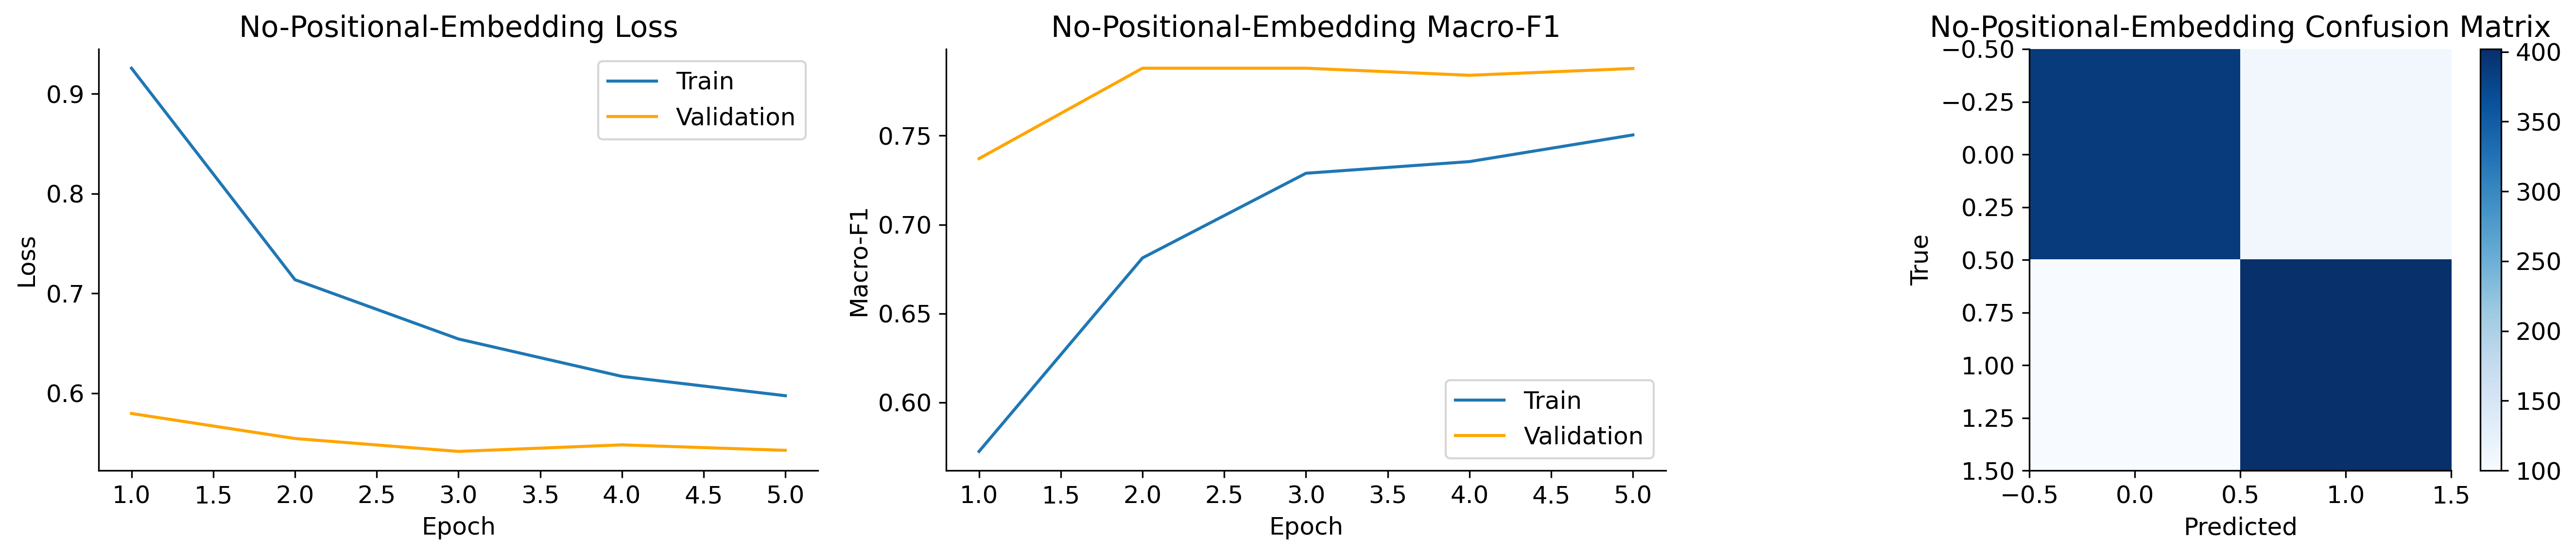
\includegraphics[width=\linewidth]{ablation_no_positional_embedding.png}
    \caption{Removing positional embeddings.}
  \end{subfigure}
  \begin{subfigure}[b]{0.45\textwidth}
    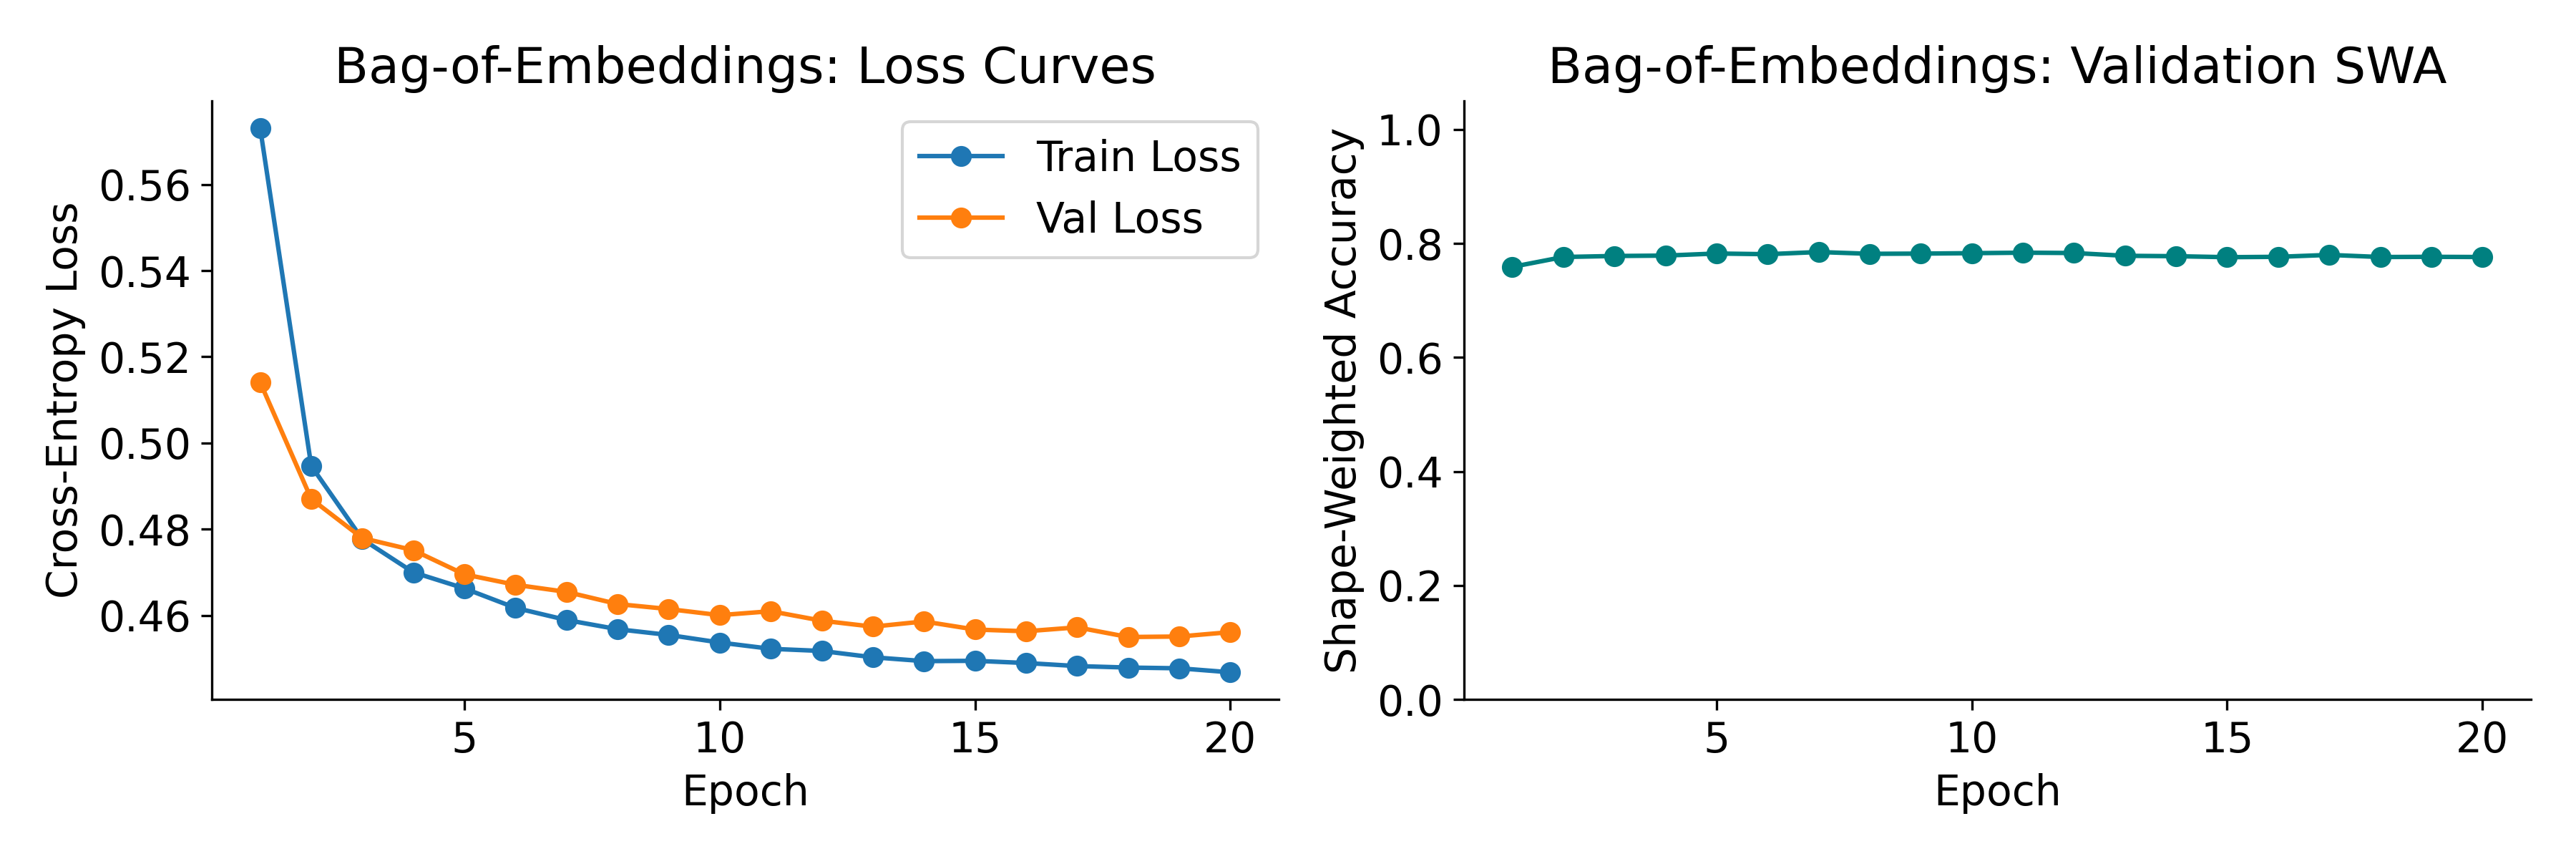
\includegraphics[width=\linewidth]{ablation_bag_of_embeddings.png}
    \caption{Bag-of-embeddings variant.}
  \end{subfigure}
  \caption{Ablation results illustrating architectural components affecting zero-shot symbolic generalization.}
\end{figure}

\bibliography{references}

\end{document}